\documentclass[a4paper,10pt]{article}
\usepackage{fontspec}
\setmainfont{Times New Roman}
\usepackage[left=1.2cm, right=1.2cm, top=1.5cm, bottom=1.5cm]{geometry}
\usepackage{enumitem}
\usepackage{titlesec}
\usepackage{xcolor}
\usepackage{hyperref}
\usepackage{graphicx}
\usepackage{tabularx}
\usepackage{ulem}
\usepackage{booktabs}
\usepackage{fontawesome5}
\usepackage{marvosym}
\usepackage{parskip}

\hypersetup{
    colorlinks=true,
    linkcolor=black,
    filecolor=black,
    urlcolor=blue,
}

\titleformat{\section}{\Large\bfseries\color{black}}{}{0em}{}
\titleformat{\subsection}{\bfseries}{}{0em}{}
\setlist[itemize]{leftmargin=*, noitemsep, topsep=1pt, parsep=0pt}
\renewcommand{\arraystretch}{1.2}

\begin{document}
\raggedbottom
\titlespacing{\section}{0pt}{6pt}{3pt}
\titlespacing{\subsection}{0pt}{4pt}{2pt}
\linespread{1.1}

\noindent
\begin{tabular}{m{3cm} l}
    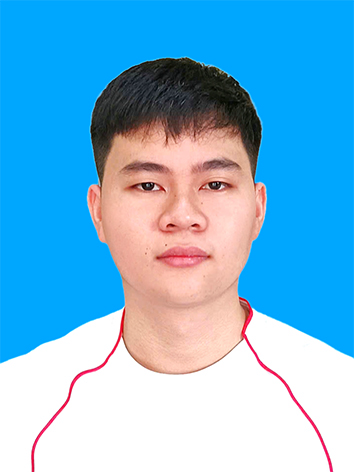
\includegraphics[width=3cm, height=3.5cm]{image.png} &
    \begin{tabular}{@{}l}
        \multicolumn{1}{c}{\textbf{\LARGE Nguyễn Hữu Lộc} \quad \textbf{\large Fresher Backend Developer}} \\[10pt]
        \begin{tabular}{@{}ll@{}}
            \faEnvelope & \href{mailto:lockbkbang@gmail.com}{\uline{lockbkbang@gmail.com}} \\
            \faPhone & 0397845443 \\
            \faBirthdayCake & 23/09/2004 \\
        \end{tabular}
        \hspace{20pt}
        \begin{tabular}{@{}ll@{}}
            \faMapMarker & Hoc Mon, Ho Chi Minh City \\
            \faGithub & \href{https://github.com/LocNguyenSGU}{\uline{https://github.com/LocNguyenSGU}} \\
            \faGlobe & \href{https://locnguyensgu.github.io/nguyenhuuloc2k4/}{\uline{https://locnguyensgu.github.io/nguyenhuuloc2k4/}} \\
        \end{tabular}
    \end{tabular}
\end{tabular}

\section{Career Objective}
\vspace{-10pt}
\noindent\rule{\linewidth}{0.5pt}
Final-year Information Technology student with a strong interest in backend development. Seeking a \textbf{Fresher Backend Developer} position to apply academic knowledge in real-world products, strengthen system design skills, and contribute effectively to an engineering team.

\section{Education}
\vspace{-10pt}
\noindent\rule{\linewidth}{0.5pt}
\begin{tabularx}{\linewidth}{l X}
    \textbf{09/2022 - 02/2026} & \textbf{Sai Gon University} \\
    & Bachelor of Information Technology \\
    & GPA: 3.38/4.0 (8.26/10) \\
    & Academic Encouragement Scholarship: 5 times
\end{tabularx}

\section{Achievements}
\vspace{-8pt}
\noindent\rule{\linewidth}{0.5pt}
\begin{itemize}
    \item \textbf{2nd Place, Hackathon 02/2025 (Sai Gon University)}: Built an AI-powered learning assistant using the \textbf{OpenAI API}; led backend development and delivered a working demo within 24 hours.
    \item \textbf{Research Paper}: \textit{Adaptive Learning Optimization for Reinforcement Learning}, published and presented in person at \textbf{FJCAI 2026} (International Artificial Intelligence Conference 2026).
    \item \textbf{Graduation Thesis}: Developed an AI-integrated Moodle system and received a \textbf{10/10} final score.
\end{itemize}

\section{Skills}
\vspace{-10pt}
\noindent\rule{\linewidth}{0.5pt}
\renewcommand{\arraystretch}{1.1}
\begin{tabularx}{\linewidth}{l X}
    \textbf{Programming Languages:} & Java, Ruby \\
    \textbf{Frameworks:} & Spring Boot, Ruby on Rails, ReactJS \\
    \textbf{Databases:} & MySQL, Redis, MongoDB, PostgreSQL \\
    \textbf{Architecture:} & Microservices, MVC \\
    \textbf{Real-time Communication:} & WebSocket \\
    \textbf{Tools / DevOps:} & Git/GitHub, Docker, AWS Cloud, n8n
\end{tabularx}

\section{Projects}
\vspace{-10pt}
\noindent\rule{\linewidth}{0.5pt}

\subsection*{1. Internal System \hfill \small (Team Project - 5 members)}
\begin{itemize}
    \item \textbf{Timeline:} 09/2025 - 09/2026
    \item \textbf{Description:} Built an internal system for managing orders, employees, customers, and products for an e-commerce business using the \textbf{MVC} architecture and \textbf{PostgreSQL}.
    \item \textbf{Key Responsibilities:}
    \begin{itemize}
        \item Developed backend features for the order management module, supporting a workload of more than \textbf{5,000 orders per day}.
        \item Implemented a price crawling and processing pipeline for e-commerce product data from large CSV files with \textbf{100,000+ rows}, using \textbf{Sidekiq} for asynchronous processing and \textbf{PostgreSQL} for storage.
        \item Migrated data from two separate databases into a unified storage system, handling complex datasets with more than \textbf{500,000 records}.
        \item Built an invoice information extraction tool for complex document formats, achieving \textbf{97\%} accuracy by integrating the \textbf{Gemini AI} API.
        \item Built an \textbf{MCP}-based automation flow and product posting bot that handled up to \textbf{1,000 products per day}, with per-product rate limiting and \textbf{create, retrieve, update} operations to improve operational efficiency.
    \end{itemize}
    \item \textbf{Technologies:} Ruby, MVC, PostgreSQL, Redis, Docker, AWS EC2, Sidekiq
\end{itemize}

\subsection*{2. SEO Content Automation System \hfill \small (Team Project - 3 members)}
\begin{itemize}
    \item \textbf{Timeline:} 12/2024 - 06/2025
    \item \textbf{Description:} Developed a system for automated SEO content generation, trend analysis, and website publishing.
    \item \textbf{Key Responsibilities:}
    \begin{itemize}
        \item Designed the overall system architecture and database structure for the content generation workflow.
        \item Built a trend-processing and article generation pipeline using \textbf{OpenAI API} and \textbf{DeepSeek}, then published content to websites through \textbf{Shopify GraphQL}.
        \item Set up \textbf{n8n} workflows and implemented real-time updates with \textbf{WebSocket}.
        \item Improved the daily content production workflow, achieving an article acceptance rate of about \textbf{80\%} and contributing to an approximately \textbf{20\%} increase in SEO traffic.
    \end{itemize}
    \item \textbf{Technologies:} Ruby, OpenAI API, DeepSeek, Shopify GraphQL, n8n, WebSocket
\end{itemize}

\end{document}
